\subsection{Services}

This problem will have you write a service for the client-service structure. 

\subsubsection{Creating a Service}\label{p:service1}

The work for this problem should be done in the file \texttt{draw\_server.py}.

\begin{figure}[h]
  \centering
  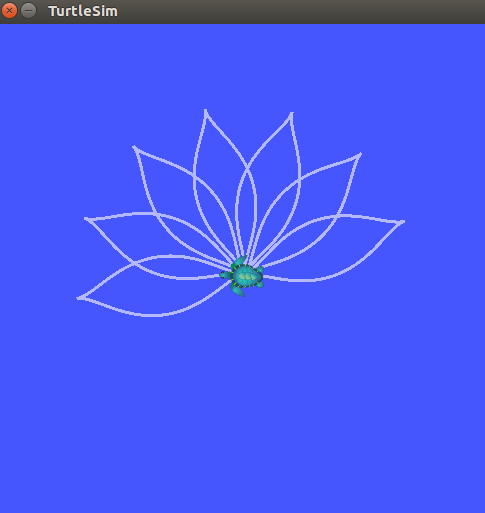
\includegraphics[width=150pt]{figures/p1/problem4a.png}
  \caption{For Problem \ref{p:service1}}
  \label{fig:3}
\end{figure}

\begin{enumerate}[(a)]
  \item In \texttt{draw}:
  \begin{enumerate}[i.]
    \item Initialize \texttt{vel\_msg}.
    \item Set $k$ to be the count parameter of \texttt{req}. %maybe this is too much hand holding idk
    \item To calculate constants, use \texttt{numpy} to perform the following operations on the
    following matrices:

    $$M_3 = \begin{bmatrix} 
      1 & 1 & 2\\
      3 & 5 & 8 \\
      13 & 21 & 34
    \end{bmatrix} 
    M_4 = \begin{bmatrix} 
      1 & 8 & 7\\
      2 & 5 & 3 \\
      9 & 2 & 6
    \end{bmatrix}$$
    
    $$a = det(M_3) -1$$
    
    $$b = -((M_3*M_4)_{(2,0)}-(M_3*M_4)_{(2,2)}) +1$$
    
    $$A = (\langle M_3, M_4 \rangle^T_{(0,0)} - \langle M_3,M_4 \rangle^T_{(1,0)})/10$$
    
    $$B = ((M_3*M_4)^T_{(2,1)}-\langle M_3,M_4 \rangle^T_{(2,1)})/2.0 $$
    
    \item Each of the above computed constants should be set as rosparams \texttt{a}, \texttt{b},
    \texttt{A}, and \texttt{B} with the type \texttt{float}.

  \end{enumerate}

  \item In \texttt{if req.rotate} section:
  \begin{enumerate}[i.]
    \item If \texttt{req.rotate}, set angular z to -3 and linear x to 0.
    \item Otherwise use \texttt{numpy} to set angular z to $B*cos(b*count)$ and linear x to $A*sin(a*count)$.
  \end{enumerate}

  \item Also be sure to return your velocity message before the end of the \texttt{draw} function.
  \item In \texttt{draw\_server}: Create a service with the name \texttt{`draw'}, service\_class
  \texttt{Draw} and handler \texttt{draw}. Please see rospy documentation for further details.
  \item In \texttt{\_\_name\_\_ == `\_\_main\_\_'}: Call your function!
  \item In \texttt{draw\_server.launch}:
  \begin{enumerate}[i.]
    \item Launch the turtlesim node.
    \item Launch \texttt{draw\_service} node from \texttt{draw\_server.py}.
    \item  Launch \texttt{draw\_flower} node from \texttt{client.py}.
  \end{enumerate}

\end{enumerate}
Your resulting flower should resemble Figure~\ref{fig:3}.

\subsubsection{Integrating the pieces}\label{p:service2}

The work for this problem should be done in file \texttt{spawn\_flower.py}. 

\begin{figure}[h]
  \centering
  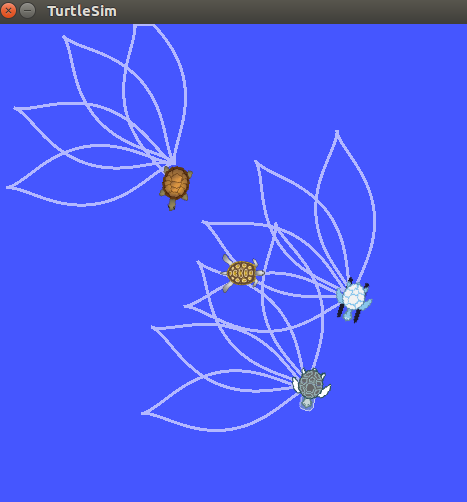
\includegraphics[width=150pt]{figures/p1/problem4b_3turts.png}
  \caption{For Problem~\ref{p:service2}}\label{fig:4}
\end{figure}

\begin{enumerate}[(a)]
  \item In \texttt{draw\_flower}:
  \begin{enumerate}[i.]
    \item Initialize your \texttt{`draw\_turtle'} node
    .
    \item Block while waiting for the \texttt{`spawn'} service to become available. See rospy
    documentation for more information.

    \item In first \texttt{try}: Create a handle for calling the spawn service.
    \item In second \texttt{try}: Follow the instructions in the comments.
    \item Block while waiting for \texttt{`/draw'} service, and then set up the service handle for
    the draw service (in the same way as problem 3). %these instructions seem vague, come back and fix

    \item Set up velocity publisher for \texttt{`{}/cmd\_vel'.format(turtle\_name)} and set the rate to 5.
  \end{enumerate}
  
  
  
  \item In \texttt{while not rospy.is\_shutdown()} section of \texttt{draw\_flower}: Publish the
  velocity messages returned from draw. Then sleep for predetermined rate.

  \item In \texttt{\_\_name\_\_ == `\_\_main\_\_'}: Call your function!
  \item In \texttt{spawn\_flower.launch}:
  \begin{enumerate}[i.]
    \item Launch the turtlesim node.
    \item Launch \texttt{draw\_service} node from \texttt{draw\_server.py}.
    \item  Launch \texttt{launcher} node from \texttt{launcher.py}.
  \end{enumerate}

  Your resulting product should resemble Figure~\ref{fig:4}. There should be between 2 and 5 turtles
  spawned, in addition to the original turtle. The starting points of the turtles is random.


\end{enumerate}

%%% Local Variables:
%%% mode: latex
%%% TeX-master: "../assessment"
%%% End:
